% \documentclass[paper=A4,fontsize=11pt]{article} % KOMA-article class
\documentclass[a4paper,fontsize=11pt]{scrartcl} % KOMA-article class
\usepackage[colorlinks=true,linkcolor=blue,urlcolor=blue]{hyperref}
% \usepackage{ctex}
% \usepackage[UTF8]{ctex}
\usepackage{xeCJK}%中文字体
\xeCJKsetup{AutoFakeSlant={true},AutoFakeBold={true}}





\usepackage{graphicx}                    % Enable pdflatex
\usepackage{wrapfig}


% \usepackage[svgnames]{xcolor}            % Colors by their 'svgnames'


\usepackage{layout} %显示布局

\setlength\hoffset{-0.25cm}
\setlength\voffset{-0cm}
\setlength\topmargin{0cm}
\setlength\headheight{2.2cm}
\setlength\headsep{0.25cm}
\setlength\oddsidemargin{0pt}
\setlength\textwidth{\paperwidth}
\addtolength\textwidth{-2in}
\setlength\textheight{\paperheight}
\addtolength\textheight{-2.8in}




\usepackage{fancyhdr}
% \frenchspacing              % Better looking spacings after periods
% \pagestyle{empty}           % No pagenumbers/headers/footers
\pagestyle{fancy}
\fancyhf{}
\rhead{
	% \vspace*{-0.25cm}
	
\includegraphics[height=2cm]{nus.png}}
\lhead{
	% \vspace*{-2cm}
	
\includegraphics[height=2cm]{hust.png}}




% % 设置默认字体及自定义命令
% \setCJKfamilyfont{song}{SimSun}                             %宋体 song  
% % \setmainfont{Times New Roman}%设置Times New Roman为默认的英文字体  
% % \setCJKmainfont{SimSun}      %设置宋体为默认的中文字体 
% % \setCJKmainfont{SimHei}      %设置宋体为默认的中文字体 
% % \setCJKmainfont{NotoSansCJK}      %设置宋体为默认的中文字体 

\setmainfont{Times New Roman}%缺省英文字体.serif是有衬线字体sans serif无衬线字体
\setCJKmainfont[ItalicFont={楷体}, BoldFont={黑体}]{宋体}%衬线字体 缺省中文字体为
% \setCJKmainfont[ItalicFont={楷体}, BoldFont={黑体}]{SimSun}%衬线字体 缺省中文字体为
\setCJKsansfont{黑体}
\setCJKmonofont{仿宋_GB2312}%中文等宽字体
%-----------------------xeCJK下设置中文字体------------------------------%
\setCJKfamilyfont{song}{SimSun}                             %宋体 song  
\newcommand{\song}{\CJKfamily{song}}                        
\setCJKfamilyfont{fs}{FangSong_GB2312}                      %仿宋2312 fs  
\newcommand{\fs}{\CJKfamily{fs}}                            
\setCJKfamilyfont{yh}{Microsoft YaHei}                    %微软雅黑 yh  
\newcommand{\yh}{\CJKfamily{yh}}  
\setCJKfamilyfont{hei}{SimHei}                              %黑体  hei  
\newcommand{\hei}{\CJKfamily{hei}}    
\setCJKfamilyfont{hwxh}{STXihei}                                %华文细黑  hwxh  
\newcommand{\hwxh}{\CJKfamily{hwxh}}
\setCJKfamilyfont{asong}{Adobe Song Std}                        %Adobe 宋体  asong  
\newcommand{\asong}{\CJKfamily{asong}}
\setCJKfamilyfont{ahei}{Adobe Heiti Std}                            %Adobe 黑体  ahei  
\newcommand{\ahei}{\CJKfamily{ahei}}  
\setCJKfamilyfont{akai}{Adobe Kaiti Std}                            %Adobe 楷体  akai  
\newcommand{\akai}{\CJKfamily{akai}}

\newcommand{\name}[1]{ % Name
\noindent\Large\textbf{#1}\normalsize\par}
\newcommand{\bfill}[1]{
	\makebox[#1]{\hfil}}
\newcommand{\stitle}[1]{
	\noindent\underline{\textbf{#1}} \normalsize\par}
	
% \setlist{nosep}

\begin{document}
% \layout % 查看页面布局是否合理
% \vspace*{+0.1cm}
\begin{wrapfigure}{r}{0.16\textwidth} %this figure will be at the right
	\vspace*{-0.42cm}
    \hfil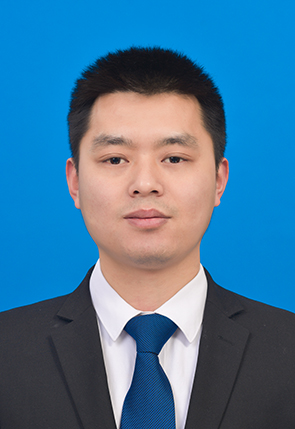
\includegraphics[width=0.16\textwidth]{yong.jpg}
\end{wrapfigure}

\name{李\quad 勇}
\noindent \textbf{联系电话:}\href{tel:+8615072423262}{(+86)150-7242-3262} \bfill{1.25cm}
\textbf{电子邮件:} \href{mailto:yongli.cv@gmail.com}{yongli.cv@gmail.com}

\noindent \textbf{性别:}男 \bfill{1.2cm}
\textbf{籍贯:}湖北恩施 \bfill{0.75cm}
\textbf{婚姻状态:}已婚 \bfill{0.2cm}
\textbf{出生年月:}1988.10

\noindent \textbf{学历:}博士 \bfill{0.8cm}
\textbf{导师:熊有伦} 院士, 杨华 教授 \bfill{1.48cm}
\textbf{政治面貌:}中共党员 

\noindent \textbf{博士论文:}基于深度学习的粒子图像测速(PIV)算法研究及应用

\noindent \textbf{研究方向:}机器学习,图像处理,图像识别,概率图,最优控制;\\
\bfill{0.66cm}智能(测量)装备研发:新型PIV测量,工业/农业视觉检测,协作机器人; 

\vspace{0.1cm}
\hrule height 0.05cm 
\vspace{0.05cm}
\hrule
\vspace{0.05cm}

\stitle{教育经历}
\begin{itemize}
	\setlength\itemsep{0.0cm}
	\item  2012.9 - 2018.3 \bfill{1cm} 
			华中科技大学 \bfill{1cm}
			机械电子信息工程\bfill{1.4cm}
			博士学位(直攻博)
	\item  2008.9 - 2012.7 \bfill{1cm}
			华中科技大学 \bfill{1cm} 
			机械设计制造及其自动化\bfill{1.7cm}
			学士学位
\end{itemize}

\stitle{工作经历}
\begin{itemize}
	\setlength\itemsep{0.0cm}
	\item 2019.9 - 2020.12 \bfill{0.8cm}
			新加坡国立大学\bfill{0.7cm}
			计算机学院(\href{https://haroldsoh.com/}{Harold Soh})\bfill{0.4cm}
			Research Fellow
 	\item 2018.5 - 2019.04\bfill{0.9cm}
			武汉库柏特科技有限公司\bfill{3.8cm}
			算法科学家
\end{itemize}

\stitle{发表论文}
\begin{enumerate}
	\setlength\itemsep{0.0cm}
	\item \textbf{Lee, Y.}, Zhang, S., Li, M., \& He, X. (2021). Blind inverse gamma correction with maximized differential entropy. \href{https://arxiv.org/abs/2007.02246}{Arxiv link}  (Signal Processing, \textbf{JCR Q1}, 中科院2区)
	\item \textbf{Lee, Y.},\& Mei, S. (2021). Diffeomorphic Particle Image Velocimetry.  \href{https://arxiv.org/abs/2108.07438}{https://arxiv.org/abs/2108. 07438} (IEEE Transactions on Instrumentation and Measurement, \textbf{JCR Q1}, 中科院2区)
	\item Chen, K., \textbf{Lee, Y.}, \& Soh, H. (2021). Multi-Modal Mutual Information (MuMMI) Training for Robust Self-Supervised Deep Reinforcement Learning. In International conference on robotics and automation (ICRA). (\textbf{共同一作},机器人顶会)
	\item \textbf{Lee, Y.}, Yang, H., \& Yin, Z. (2017). PIV-DCNN: Cascaded deep convolutional neural networks for particle image velocimetry. Experiments in Fluids,58(12), 171. \href{https://link.springer.com/article/10.1007/s00348-017-2456-1}{https://link.springer.com/article/ 10.1007/s00348-017-2456-1}(\textbf{JCR Q2}, 中科院2区)
	\item \textbf{Lee, Y.}, Yang, H., \& Yin, Z. (2017). Outlier detection for particle image velocimetry data using a locally estimated noise variance. Measurement Science and Technology,28(3), 035301. \href{https://iopscience.iop.org/article/10.1088/1361-6501/aa5431/pdf}{https://iopscience.iop.org/article/10.1088/1361-6501/aa5431/pdf}(\textbf{JCR Q2}, 中科院3区)
	\item Yang, H., Chen, L., Chen, Y., \textbf{Lee, Y.}, \& Yin, Z. (2016). Automatic barcode recognition method based on adaptive edge detection and a mapping model. Journal of Electronic Imaging,25(5), 05. (\textbf{JCR Q4},中科院4区)
	\item \textbf{Lee, Y.}, Yang, H., \& Yin, Z. (2017). Convolutional neural networks to measure the velocity gradients of particle image pairs, In The 12th international symposium on particle image velocimetry (\textbf{国际会议报告})
\end{enumerate}

\stitle{在审论文}
\begin{enumerate}
	\item \textbf{Lee, Y.}, Gu, F.,\& Gong, Z. (2021). Surrogate-based cross-correlation for particle image velocimetry. (IEEE Transactions on Instrumentation and Measurement, \textbf{JCR Q1}, 中科院2区)
	\item Gu, F., \textbf{Lee, Y.}, \& et al. (2021). Enabling Deep Learning for Asynchronous Event-based Data.  (CVPR2022, \textbf{CCF A})
	\item Hu, Y., \textbf{Lee, Y.}, \& et al. (2021). A Comprehensive Survey on Industrial Intelligence in Smart Manufacturing.  (Proceedings of the IEEE, \textbf{JCR Q1}, IF 10.96)
\end{enumerate}

\stitle{中国专利}
\begin{enumerate}
	\setlength\itemsep{0.0cm}
	\item 杨华,\textbf{李勇},尹周平,熊有伦,张步阳,钟强龙,梅爽(2013). 一种用于增强激光亮度的光学组件及高频脉冲激光光源. \href{https://patents.google.com/patent/CN103592766B}{https://patents.google.com/patent/CN103592766B}
	\item 杨华,尹周平,熊有伦,梅爽,钟强龙,张步阳,\textbf{李勇}.(2013). 一种流场实时精确测量系统及方法. \href{https://patents.google.com/patent/CN103698554B}{https://patents.google.com/patent/CN103698554B}
	% \item 杨华,尹周平,熊有伦,梅爽,钟强龙,张步阳,\textbf{李勇}.(2013). 一种流场实时精确测量系统. \href{https://patents.google.com/patent/CN203798822U}{https://patents.google.com/patent/CN203798822U}
\end{enumerate}
% \newpage

\stitle{科研/项目经历}
\begin{enumerate}
	\setlength\itemsep{0.0cm}
	\item \textbf{多模态环境动态感知与人机协作} \hfill \textit{(2019.9- 2020.12)}\\
	\textbf{支持项目:}A*STAR新加坡国家机器人研究基金(S\$1,717,000.00, 参与)\\
    \textbf{主要工作及成果:}针对智能装备(机器人)自我探索(认识环境)和在人机协作中策略优化等前沿问题,提出了
    % (a)基于变分推断方法,结合最优控制约束,直接从原始多模态传感数据中学习获得隐空间动力学(dynamics);
	(a)基于变分推断方法,结合互信息目标函数,直接从原始多模态不完全传感数据中获得隐空间动力学(dynamics),提高有模型强化学习(MBRL)的表现性能;
    (b)在概率图模型上,结合最优控制约束,学习隐空间动力学,使得模型预测控制(MPC)算法在高维观测数据上能够有效工作,成果在进一步整理中。
    \item \textbf{基于深度学习的粒子图像测速技术(PIV)研究}\hfill \textit{(2013.9-2018.12)}\\
	\textbf{支撑项目1:}国基仪器重大专项,高超音速流场实时精确测量系统研制与应用(主要成员)\\
	\textbf{支撑项目2:}国基面上项目,高超音速流场粒子图像测速示踪机理研究与应用(参与)\\
	\textbf{主要工作及成果:}基于PIV测量误差理论,结合机器学习方法,从速度场测量,速度梯度场测量及测量异常值检测替换三方面对PIV研究。(a)提出基于深度卷积神经网络的PIV速度场估计算法,提升PIV速度场的测量精度(湍流小涡结构测量)。(b)提出DCNN回归模型的PIV速度梯度场算法,显著提升流体微元的运动变形量和旋转量的测量精度。(c)利用贝叶斯混合概率建模,显著提升PIV异常值的检测精度和流场重构精度。
\item \textbf{液晶屏幕自动光学检测软件算法研发}\hfill	\textit{(2016.9-2018.12)}\\
\textbf{支撑项目:}湖北省技术创新专项重大项目, TFT-LCD光学自动检测装备研发(参与)\\
\textbf{主要工作:}针对液晶显示屏幕Mura缺陷的自动光学检测(AOI),参与视觉部分技术规划(光照不均去除、背景纹理抑制、缺陷检测等)。提出了多尺度加噪稀疏自编码对缺陷图像重构,执行缺陷检测。参与了视觉注意力机制的缺陷分类算法研究。
\item \textbf{视觉软件包条码识别模块及OCR模块研究}\hfill \textit{(2013.9-2014.6)}\\
\textbf{支撑项目:}广东省创新科研团队项目, 智能制造新型感知技术与装备(主要成员)\\
\textbf{主要工作及成果:}利用图像处理对条形码/工业字符进行检测和识别,对条码非线性变形数学建模分析实现复杂条件下1D条码鲁棒识别算法,成果发表SCI论文一篇。
% \item \textbf{双目视觉结构光测量研究	}\hfill \textit{(2011.10-2012.09)}\\
% \textbf{支撑项目:}本科毕业设计,实验室自研项目(主要成员)\\
% \textbf{主要工作及成果:}利用双目结构光对工业零件三维形貌测量,研究了结构光相位图片的相位解析及图像矫正核心算法,在标准球测量中达到0.05mm的测量精度。
\end{enumerate}



\stitle{教学科研相关事务}
\begin{enumerate}
	\setlength\itemsep{0.0cm}
	\item 参与数字制造装备与技术国家重点实验室多项国家级/省级\textbf{课题申报}及材料撰写;
	\item 华中科技大学国际本科生的《数字电路》《计算机图形学》等英文\textbf{课程助教};
	\item 国际期刊和国际会议的\textbf{审稿工作},包括Experiments in Fluids, NIPS, ICRA, ICIRA等;
\end{enumerate}

% \stitle{主要奖励及职务}
% 国家励志奖学金、校级优秀党员、校级三好研究生等;
% 班团支书、学生党支部书记、实习队长(广东华中科技大学工业技术研究院)等。

\stitle{参加学术会议}
\begin{enumerate}
	\setlength\itemsep{0.0cm}
	\item 2021 IEEE International Conference on Robotics and Automation (ICRA), 中国西安,30/5/21-5/6/21, (现场报告).
	\item The 12th International Symposium on Particle Image Velocimetry (ISPIV), 韩国釜山, 18/6/17-22/6/17, (现场报告).	
\end{enumerate}

% \stitle{专业技能}
% \begin{itemize}
% 		\setlength\itemsep{0.0cm}
% 		% \item \textbf{3D建模:} 	Inventor($\star\star\star$), CATIA($\star\star$), AutoCAD($\star$), Ansys($\star$), 等.
% 		\item \textbf{工具软件:}	Inventor($\star\star\star$), CATIA($\star\star$), AutoCAD($\star$), Ansys($\star$), \LaTeX($\star\star\star$), Origin($\star$), 等.
% 		% \item \textbf{编程语言:} 	Matlab($\star\star\star$), Python($\star\star\star$), C/C++($\star\star$), 等.
% 		\item \textbf{编程语言:}	Python($\star\star\star$), Matlab($\star\star\star$), C/C++($\star\star$), OpenCV($\star\star\star$), Pytorch($\star\star\star$), Caffe($\star$), 等.
% \end{itemize}



% \end{CJK}
\end{document}

